\section{84 -- Largest Rectangle in Histogram}
Given $n$ non-negative integers representing the histogram's bar height where the width of each bar is 1, find the area of largest rectangle in the histogram.
\begin{figure}[H]
\begin{tikzpicture}
\draw (0,0) rectangle ++(1,2);
\draw (1,0) rectangle ++(1,1);
\draw (2,0) rectangle ++(1,5);
\draw (3,0) rectangle ++(1,6);
\draw (4,0) rectangle ++(1,2);
\draw (5,0) rectangle ++(1,3);
\node at (0.5,2.3) {2};
\node at (1.5,1.3) {1};
\node at (2.5,5.3) {5};
\node at (3.5,6.3) {6};
\node at (4.5,2.3) {2};
\node at (5.5,3.3) {3};
\end{tikzpicture}
\end{figure}
Above is a histogram where width of each bar is 1, given height $H = (2,1,5,6,2,3)$.
\begin{figure}[H]
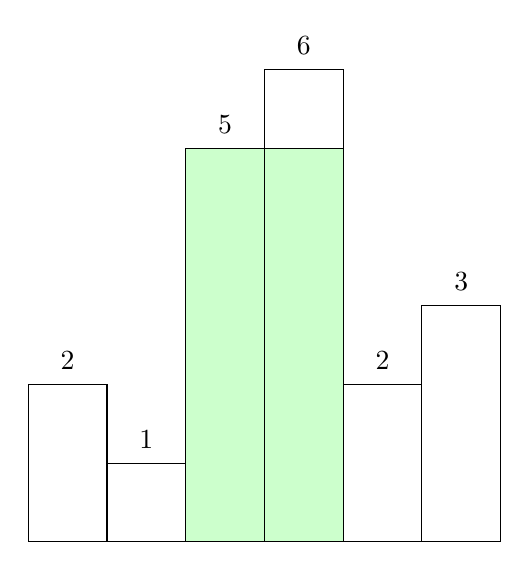
\begin{tikzpicture}

\draw (0,0) rectangle ++(1,2);
\draw (1,0) rectangle ++(1,1);
\fill[green!20!white] (2,0) rectangle ++(2,5);
\draw (2,0) rectangle ++(1,5);
\draw (3,0) rectangle ++(1,5);
\draw (3,0) rectangle ++(1,6);
\draw (4,0) rectangle ++(1,2);
\draw (5,0) rectangle ++(1,3);
\node at (0.5,2.3) {2};
\node at (1.5,1.3) {1};
\node at (2.5,5.3) {5};
\node at (3.5,6.3) {6};
\node at (4.5,2.3) {2};
\node at (5.5,3.3) {3};
\end{tikzpicture}
\end{figure}
The largest rectangle is shown in the light green area, which has area $A= 10$ unit.
\subsection{Stack Based Approach}
\begin{CJK*}{UTF8}{gbsn}
直方图中每个bar的宽度是1,对于每一个bar $x$, 需要计算出以$x$的高度作为最小高度所围起来的矩形的面积。那么如何计算出这样的面积呢?我们需要找到在$x$左边 找到第一个高度小于$x$高度的bar的index $\alpha$,同时在$x$右边找到第一个高度小于$x$高度的bar的index $\beta$。
\par
从左到右遍历直方图高度数组 $H$,同时maintain一个stack $S$。 每个bar的index都会被push到这个stack中一次。如果发现当前bar的高度比栈顶小,就把stack中比当前bar还要高的bar弹出stack。每弹出一个bar,就计算出以弹出bar作为最小高度所能围起来的矩形的面积。那么如何得到$\alpha$和$\beta$这两个index呢?其实当前的index就是$\beta$,而stack中栈顶元素的下一个元素就是$\alpha$。这样矩形的宽度就是$(\beta-1) - (\alpha+1) + 1 = \beta-\alpha$。
\par
详细的算法步骤如下:
\begin{enumerate}
\item Create 一个空栈 $S$
\item 从index $i=0$开始,
\begin{enumerate}
\item 如果$S$为空,或者当前bar的高度$H[i]$大于栈顶的bar的高度,push $i$ 到 $S$中。
\item 如果当前bar的高度$H[i]$小于栈顶的bar的高度,就remove 栈顶的bar直到栈为空或者栈顶元素小于当前高度。假设remove的栈顶元素为$H[j]$。计算出以$H[j]$为最小高度所能围起来的矩形的面积。宽度需要找到$\alpha$和$\beta$。其中$\alpha$就是栈中紧邻$j$的元素,而$\beta$就是$i$。 因此宽度即为$\beta-\alpha-1$。如果栈为空,表明左边都是大于$H[j]$的bar,这时候宽度就是$\beta-1-0+1 = \beta$\label{84step21}
\end{enumerate}
\item 如果遍历完后,栈仍不为空,继续remove掉所有栈中的bar的index,并重复[\ref{84step21}]
\end{enumerate}
\end{CJK*}
\subsection{Code}
Procedure \texttt{LargestRectangleArea} gets the maximum rectangle area can be formed for a given height array $H$ with length $L$
\setcounter{algorithm}{0}
\begin{algorithm}[H]
\caption{Stack Based Approach}
\label{84MainProc}
\begin{algorithmic}[1]
\Procedure{LargestRectangleArea}{$H, L$}
\State $S:=\emptyset$ \Comment The empty stack
\State $i:=0$
\State $A:=0$ \Comment The maximum area overall
\While{$i < n$}
\If{$S=\emptyset$ \textbf{or} $H[S[0]]\leq H[i]$}
\State $S\gets S+i$ \Comment Push index $i$ to $S$
\State $i\gets i+1$
\Else
\State $j:=S[0]$ \Comment Get the top element of $S$
\State $S\gets S\setminus S[0]$ \Comment Pop top of $S$
\State $\alpha:=-1$ \Comment If $S$ is empty, all bars in the left of $H[j]$ are higher than $H[j]$
\algstore{84algo}
\end{algorithmic}
\end{algorithm}
\begin{algorithm}[H]
\begin{algorithmic}[1]
\algrestore{84algo}
\If{$S\neq \emptyset$}
\State $\alpha\gets S[0]$ \Comment  The index of the first bar less than $H[j]$ in the left
\EndIf
\State $\theta:=H[j]\times(i - \alpha - 1)$ \Comment Area of rectangle formed with $H[j]$ as the minimum height.
\State $A\gets \max(A, \theta)$
\EndIf
\EndWhile
\While{$S\neq \emptyset$}
\State $j:=S[0]$ \Comment Get the top element of $S$
\State $S\gets S\setminus S[0]$ \Comment Pop top of $S$
\State $\alpha:=-1$ \Comment If $S$ is empty, all bars in the left of $H[j]$ are higher than $H[j]$
\If{$S\neq \emptyset$}
\State $\alpha\gets S[0]$ \Comment  The index of the first bar less than $H[j]$ in the left
\EndIf
\State $\theta:=H[j]\times(L - \alpha - 1)$ \Comment Area of rectangle formed with $H[j]$ as the minimum height. \label{84note1}
\State $A\gets \max(A, \theta)$
\EndWhile
\State \Return $A$
\EndProcedure
\end{algorithmic}
\end{algorithm}
Note: line [\ref{84note1}] uses $L$ because currently we have scanning all heights and now $i=L$